\chapter{广雅的学习}
\label{chap:study}

  \section{关于分科}
    相信很多高一新入学的学生都对自己高一下的选科、分科有很多疑惑。
  
  \section{打印在读证明}
    在读证明有很大的用处，可以向 Jetbrains 申请学生优惠和一些学生免费，也可以去广州大剧院半价看戏。打印在读证明比较方便的方式为自行打印，有两台机可以打印：一楼书吧和四楼高三书吧。如\cref{fig:prove1}为高三书吧的打印机
    \begin{figure}[ht]
      \centering
      \begin{minipage}{0.45\textwidth}
        \centering
        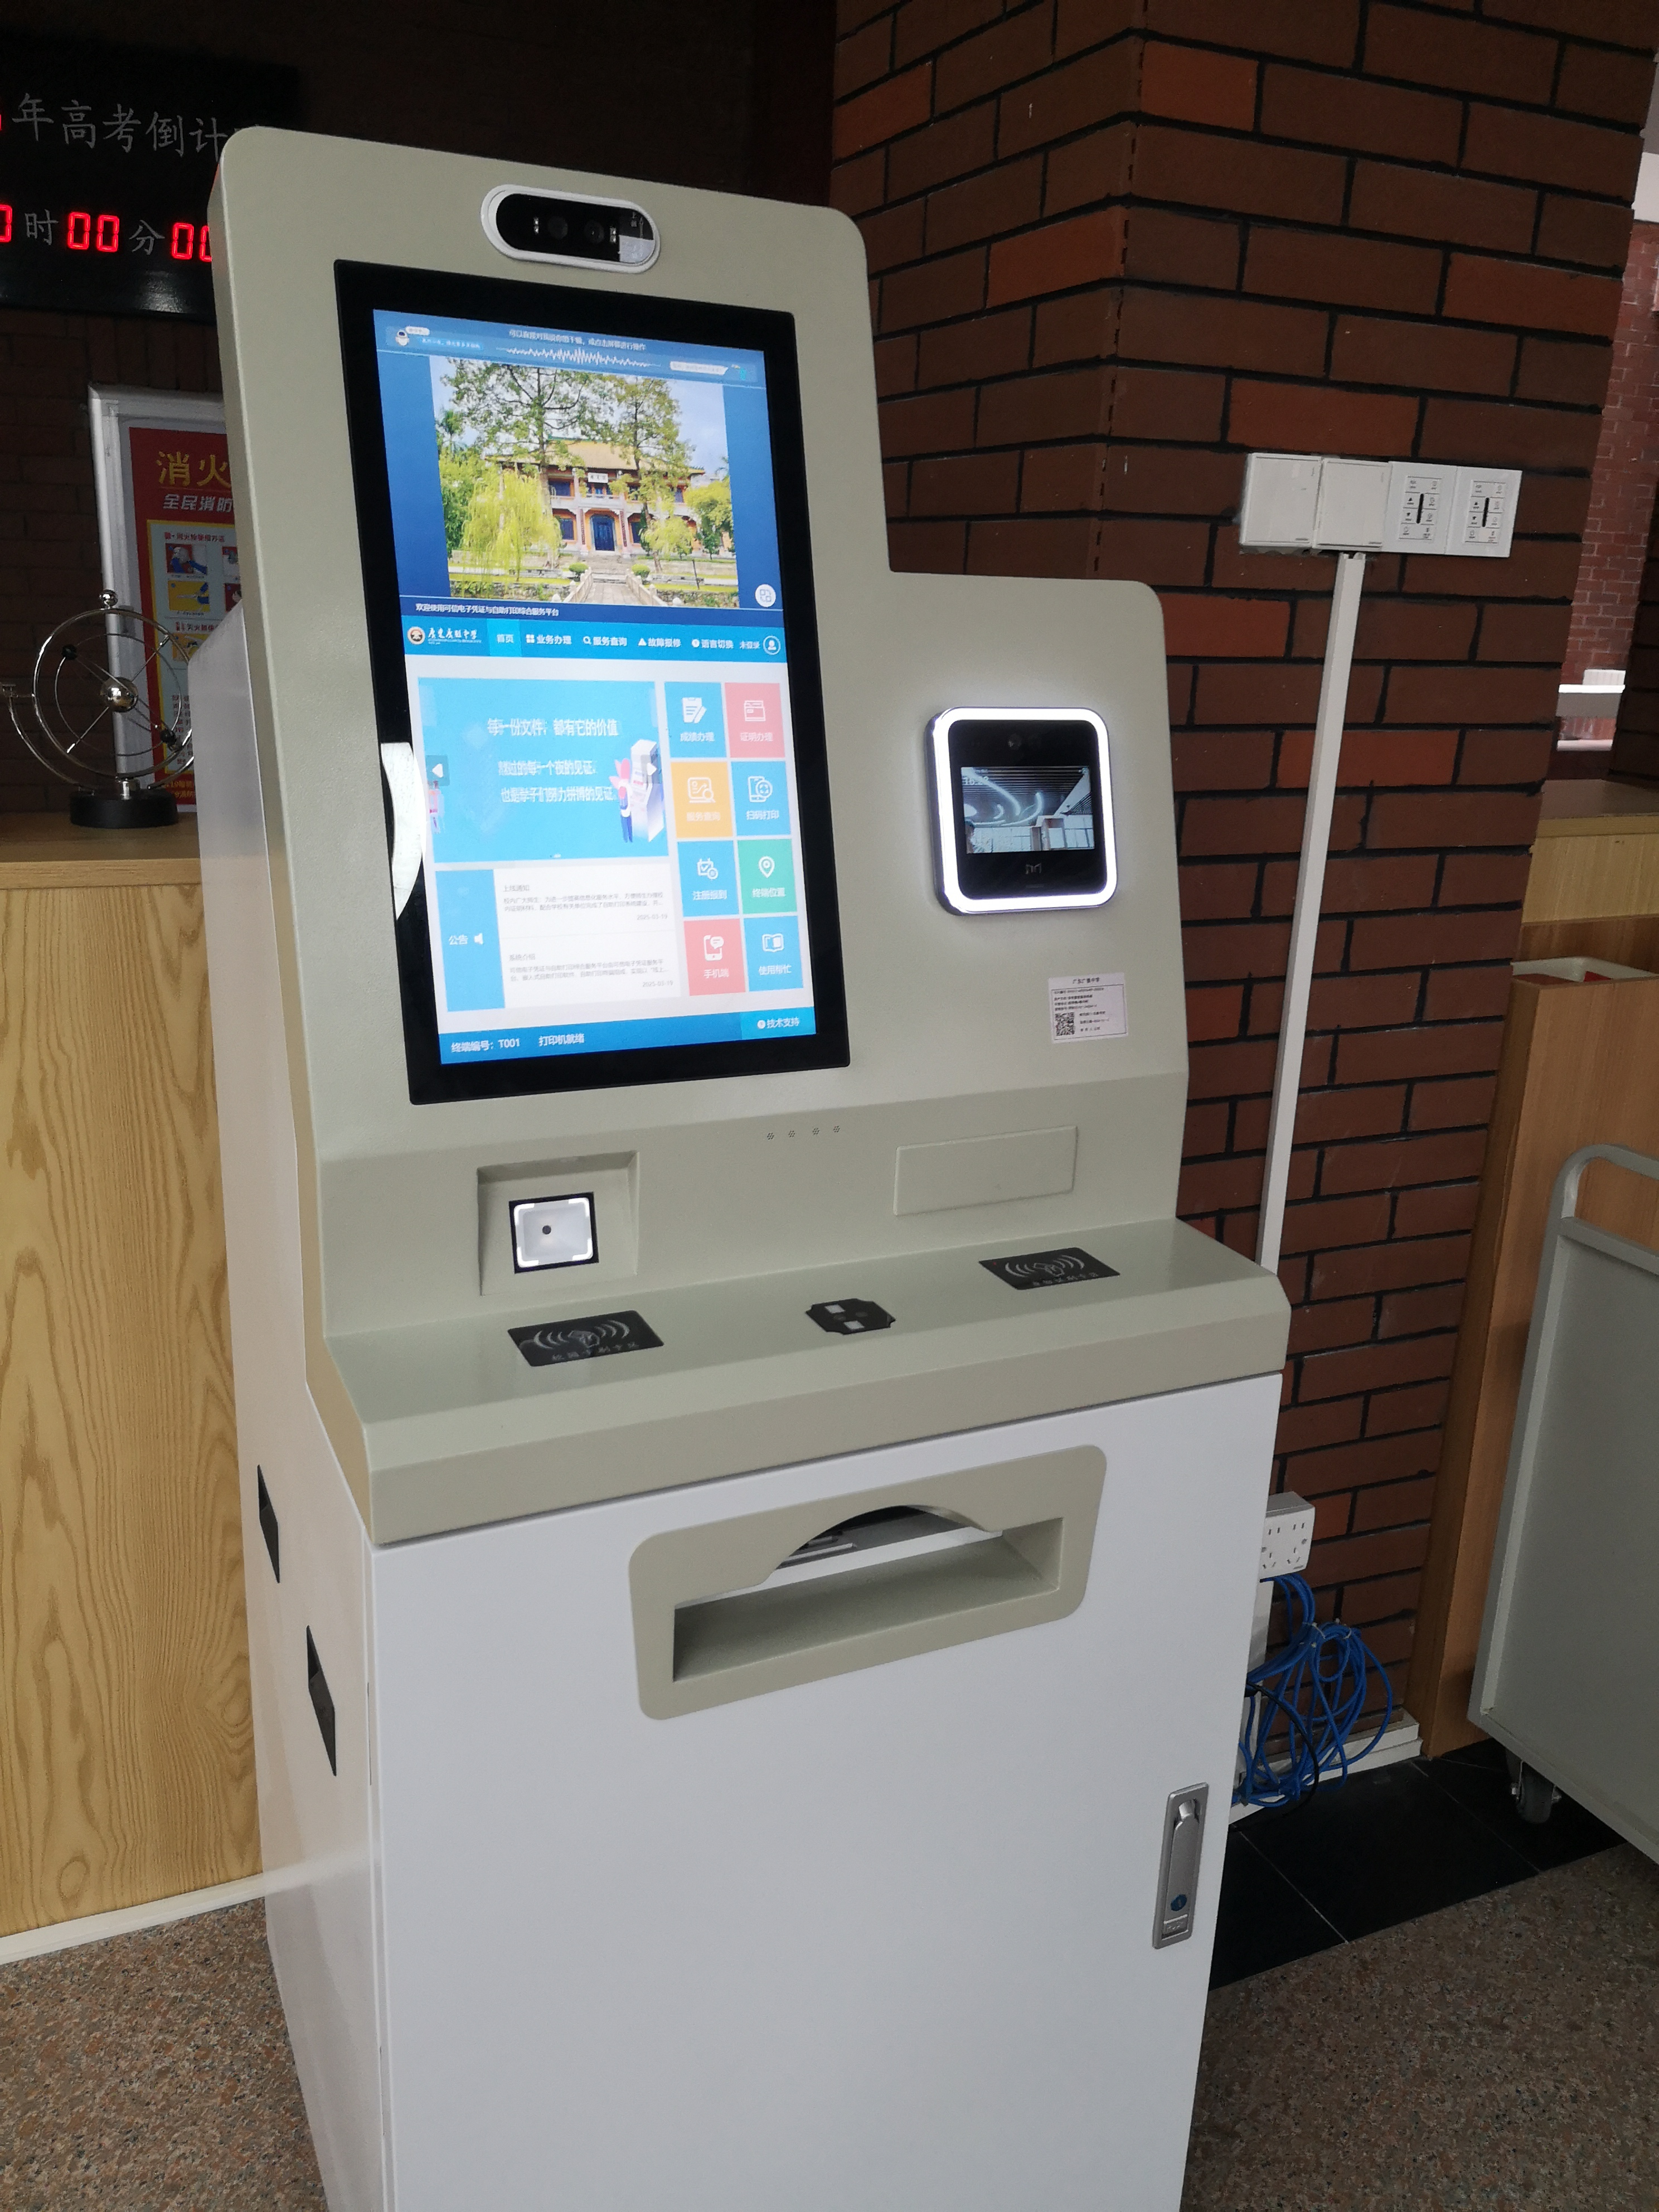
\includegraphics[width=\textwidth]{prove/prove1}
        \caption*{打印机}
        \label{fig:prove1}
      \end{minipage}
      \hfill
      \begin{minipage}{0.45\textwidth}
        \centering
        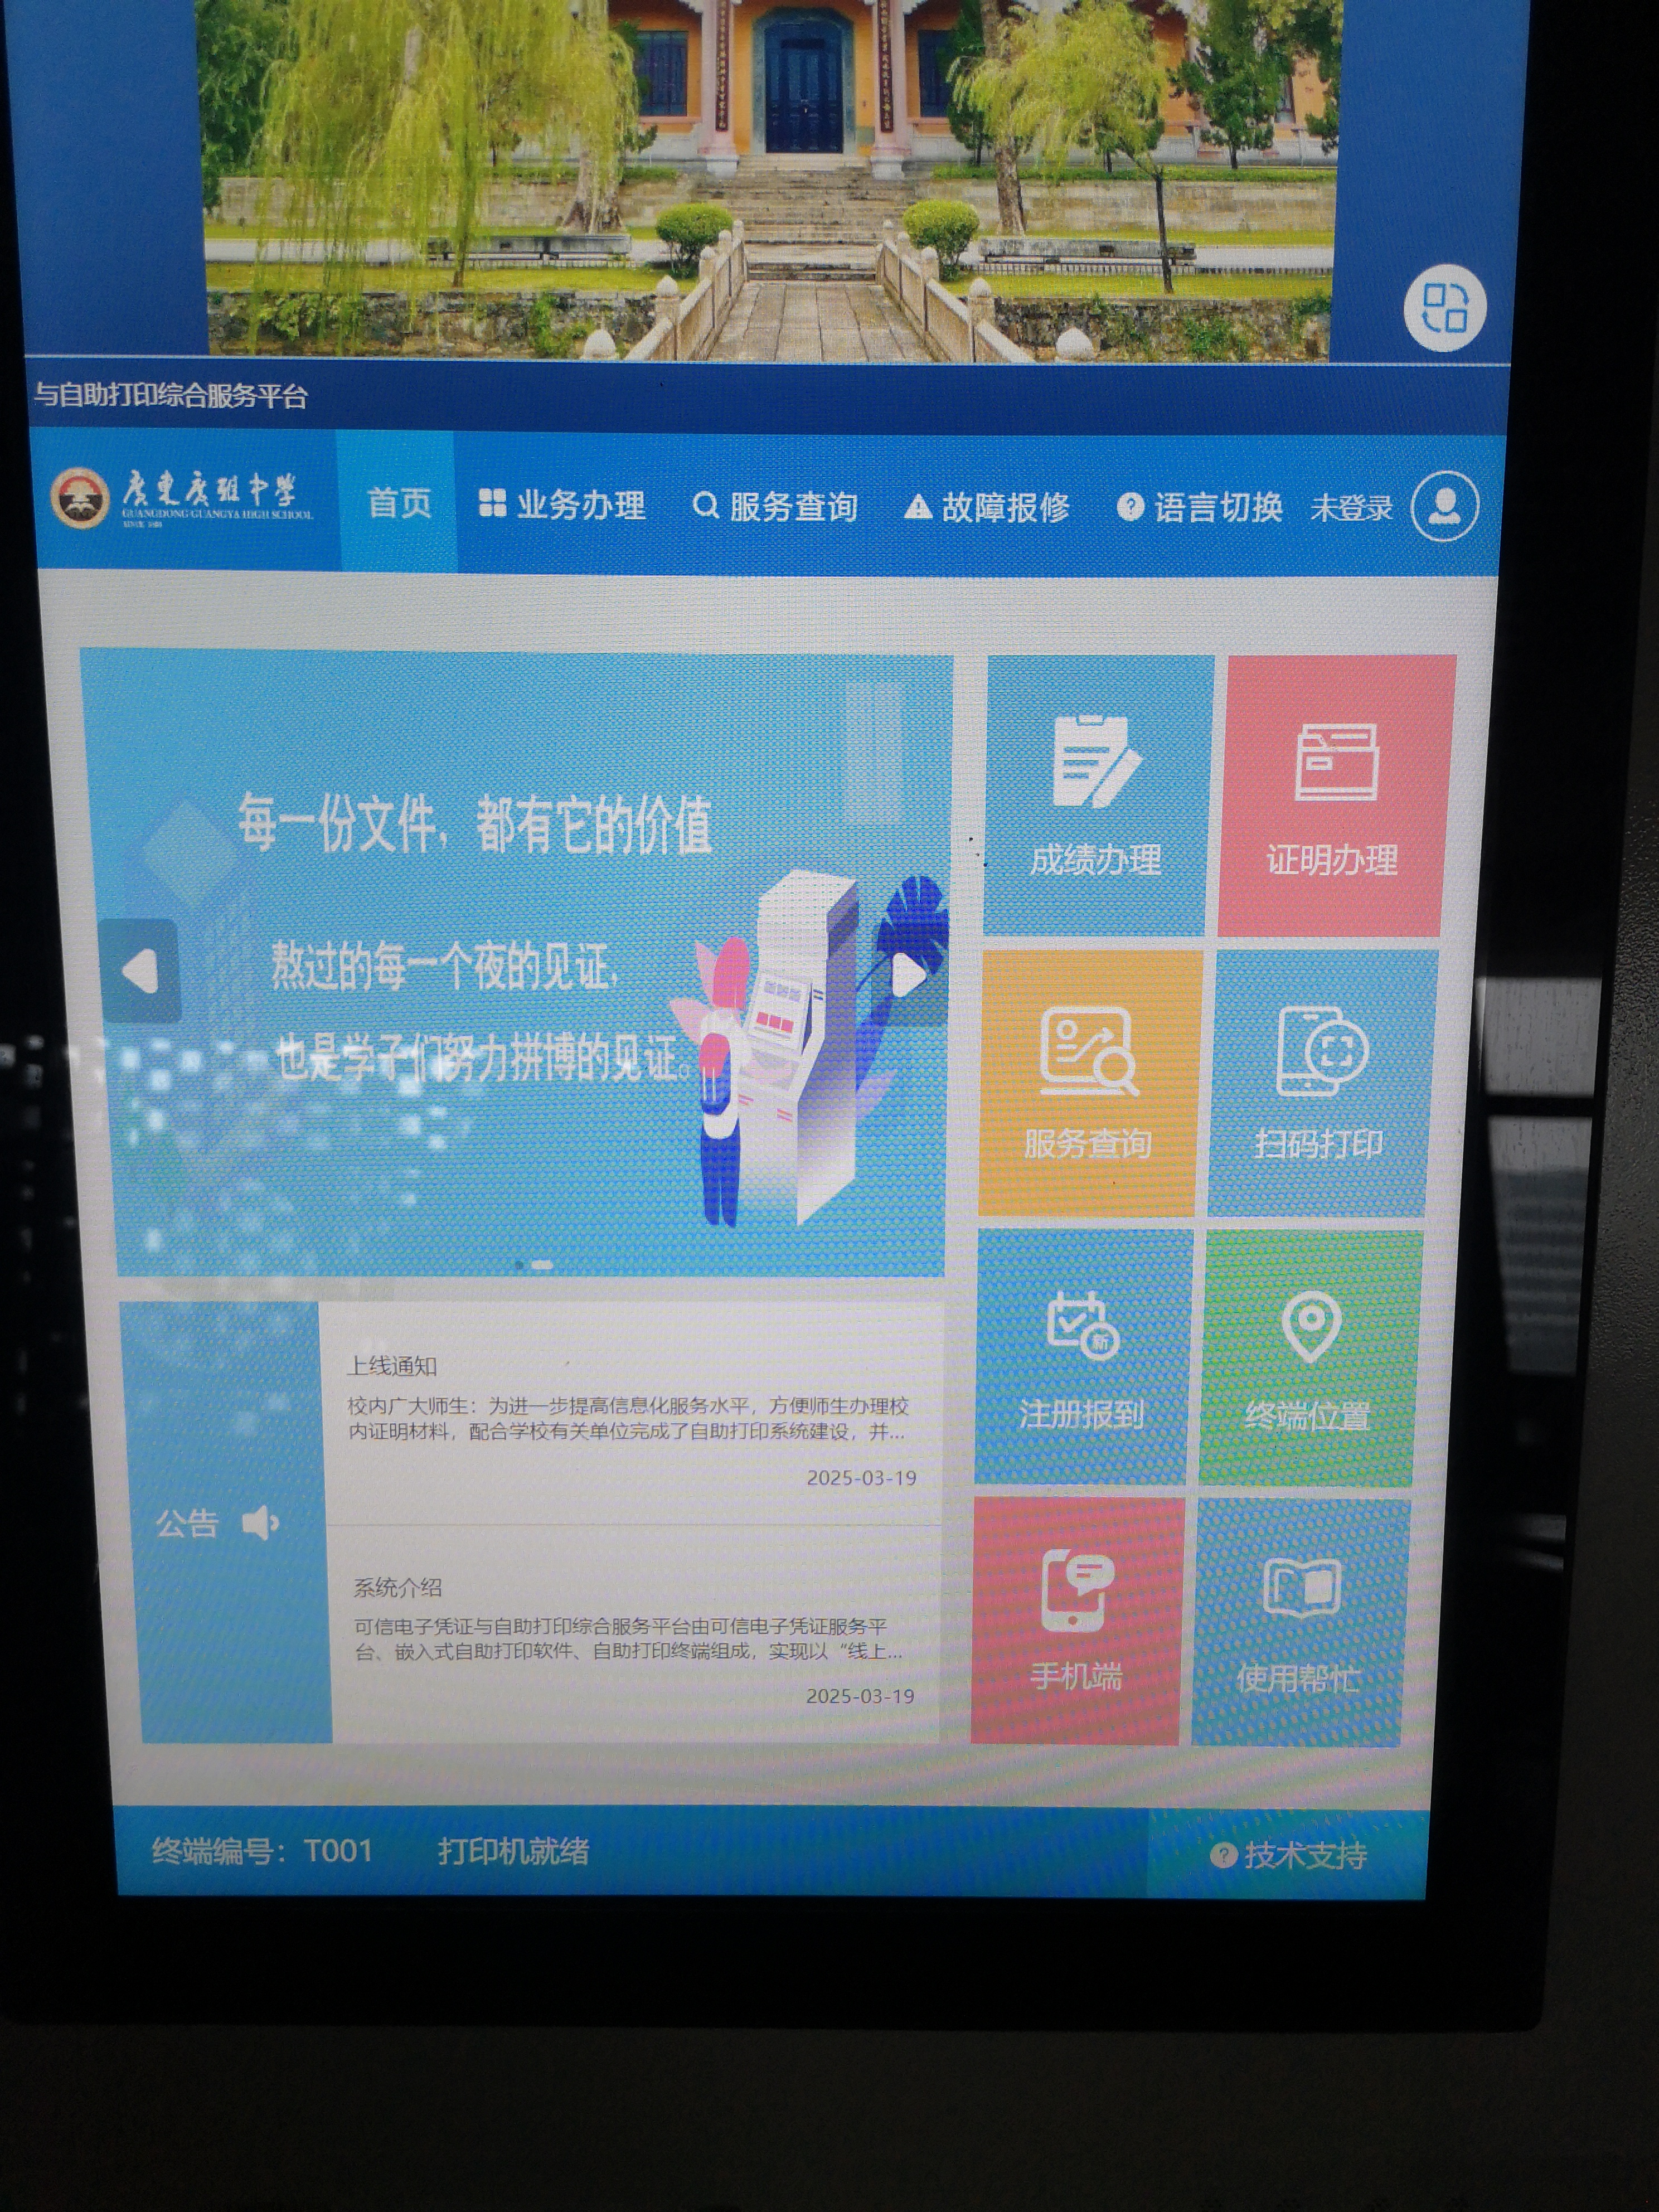
\includegraphics[width=\textwidth]{prove/prove2}
        \caption*{打印机屏幕}
        \label{fig:prove2}
      \end{minipage}
    \end{figure}
    我们可以点击右上角的“登录”来登录你的账号。什么？你不知道自己的账号是什么？没关系，点开后的登录方式选择“账号密码”，如\cref{prove3}。然后填写你的学号和身份证后6位，如\cref{prove4}。不出意外，没被别人改过得话，点击“登录”按钮就可以登录了。
    \begin{figure}[ht]
      \centering
      \begin{minipage}{0.45\textwidth}
        \centering
        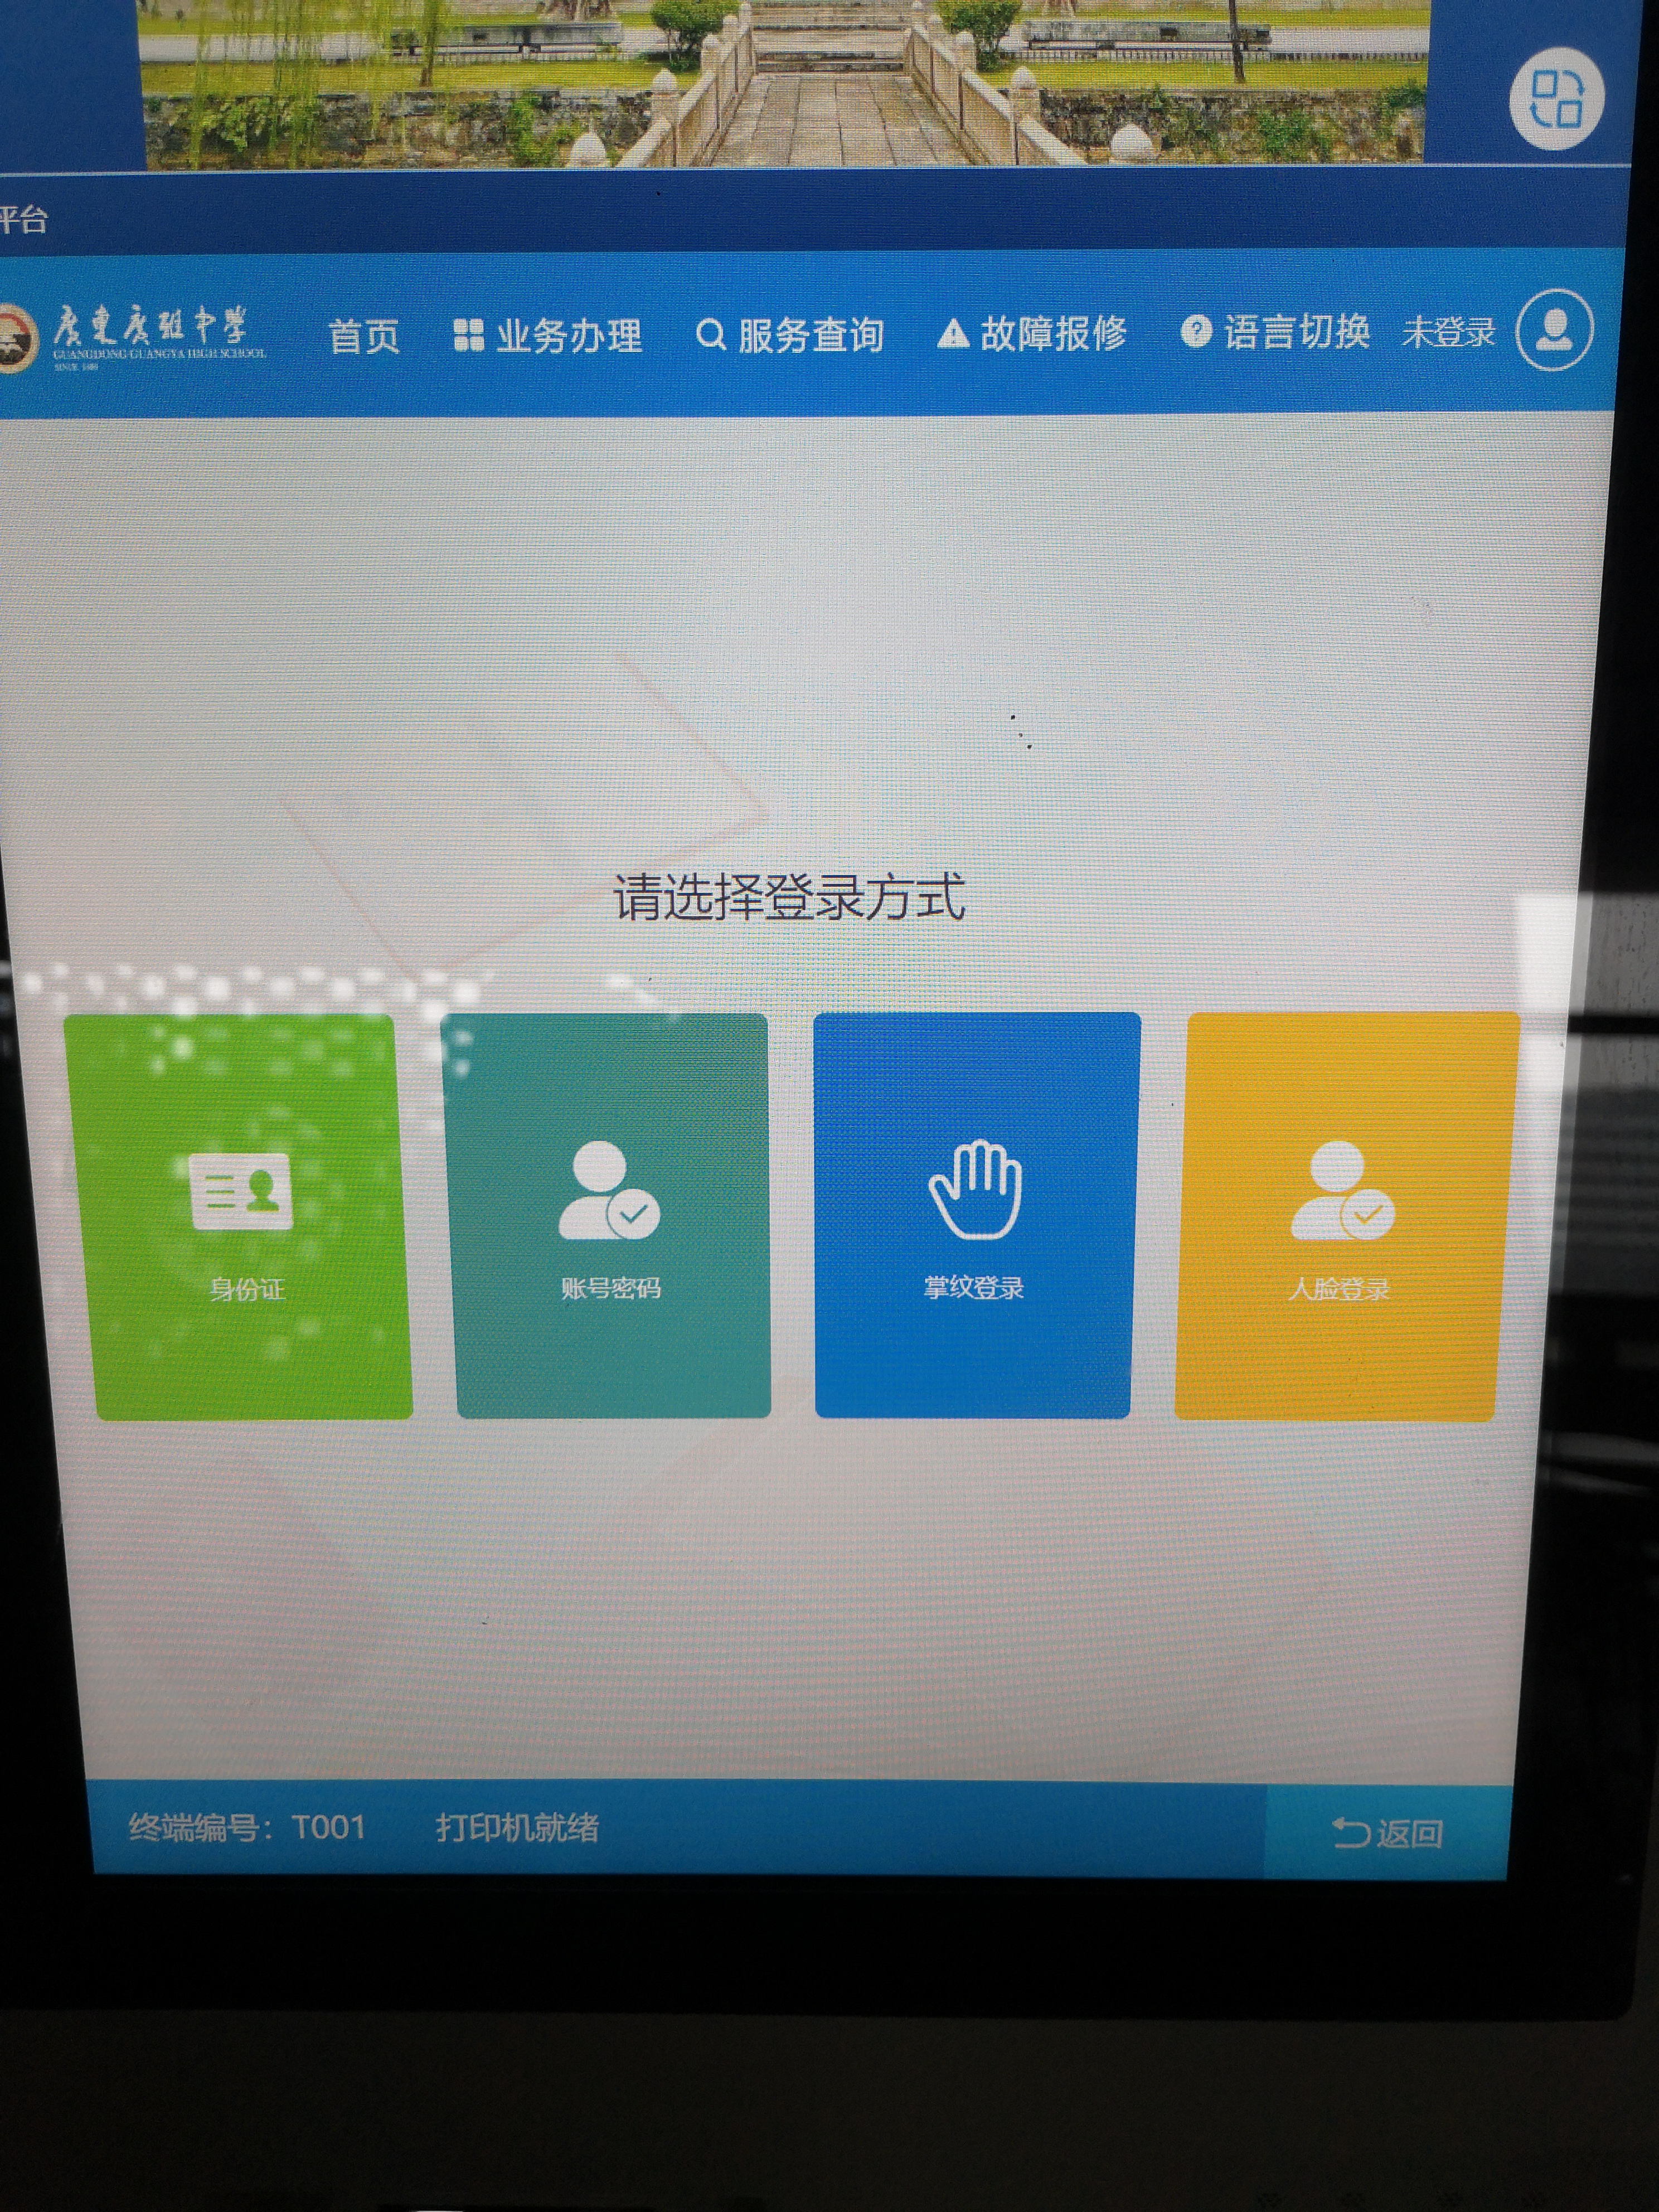
\includegraphics[width=\textwidth]{prove/prove3}
        \caption*{选择登录方式}
        \label{fig:prove3}
      \end{minipage}
      \hfill
      \begin{minipage}{0.45\textwidth}
        \centering
        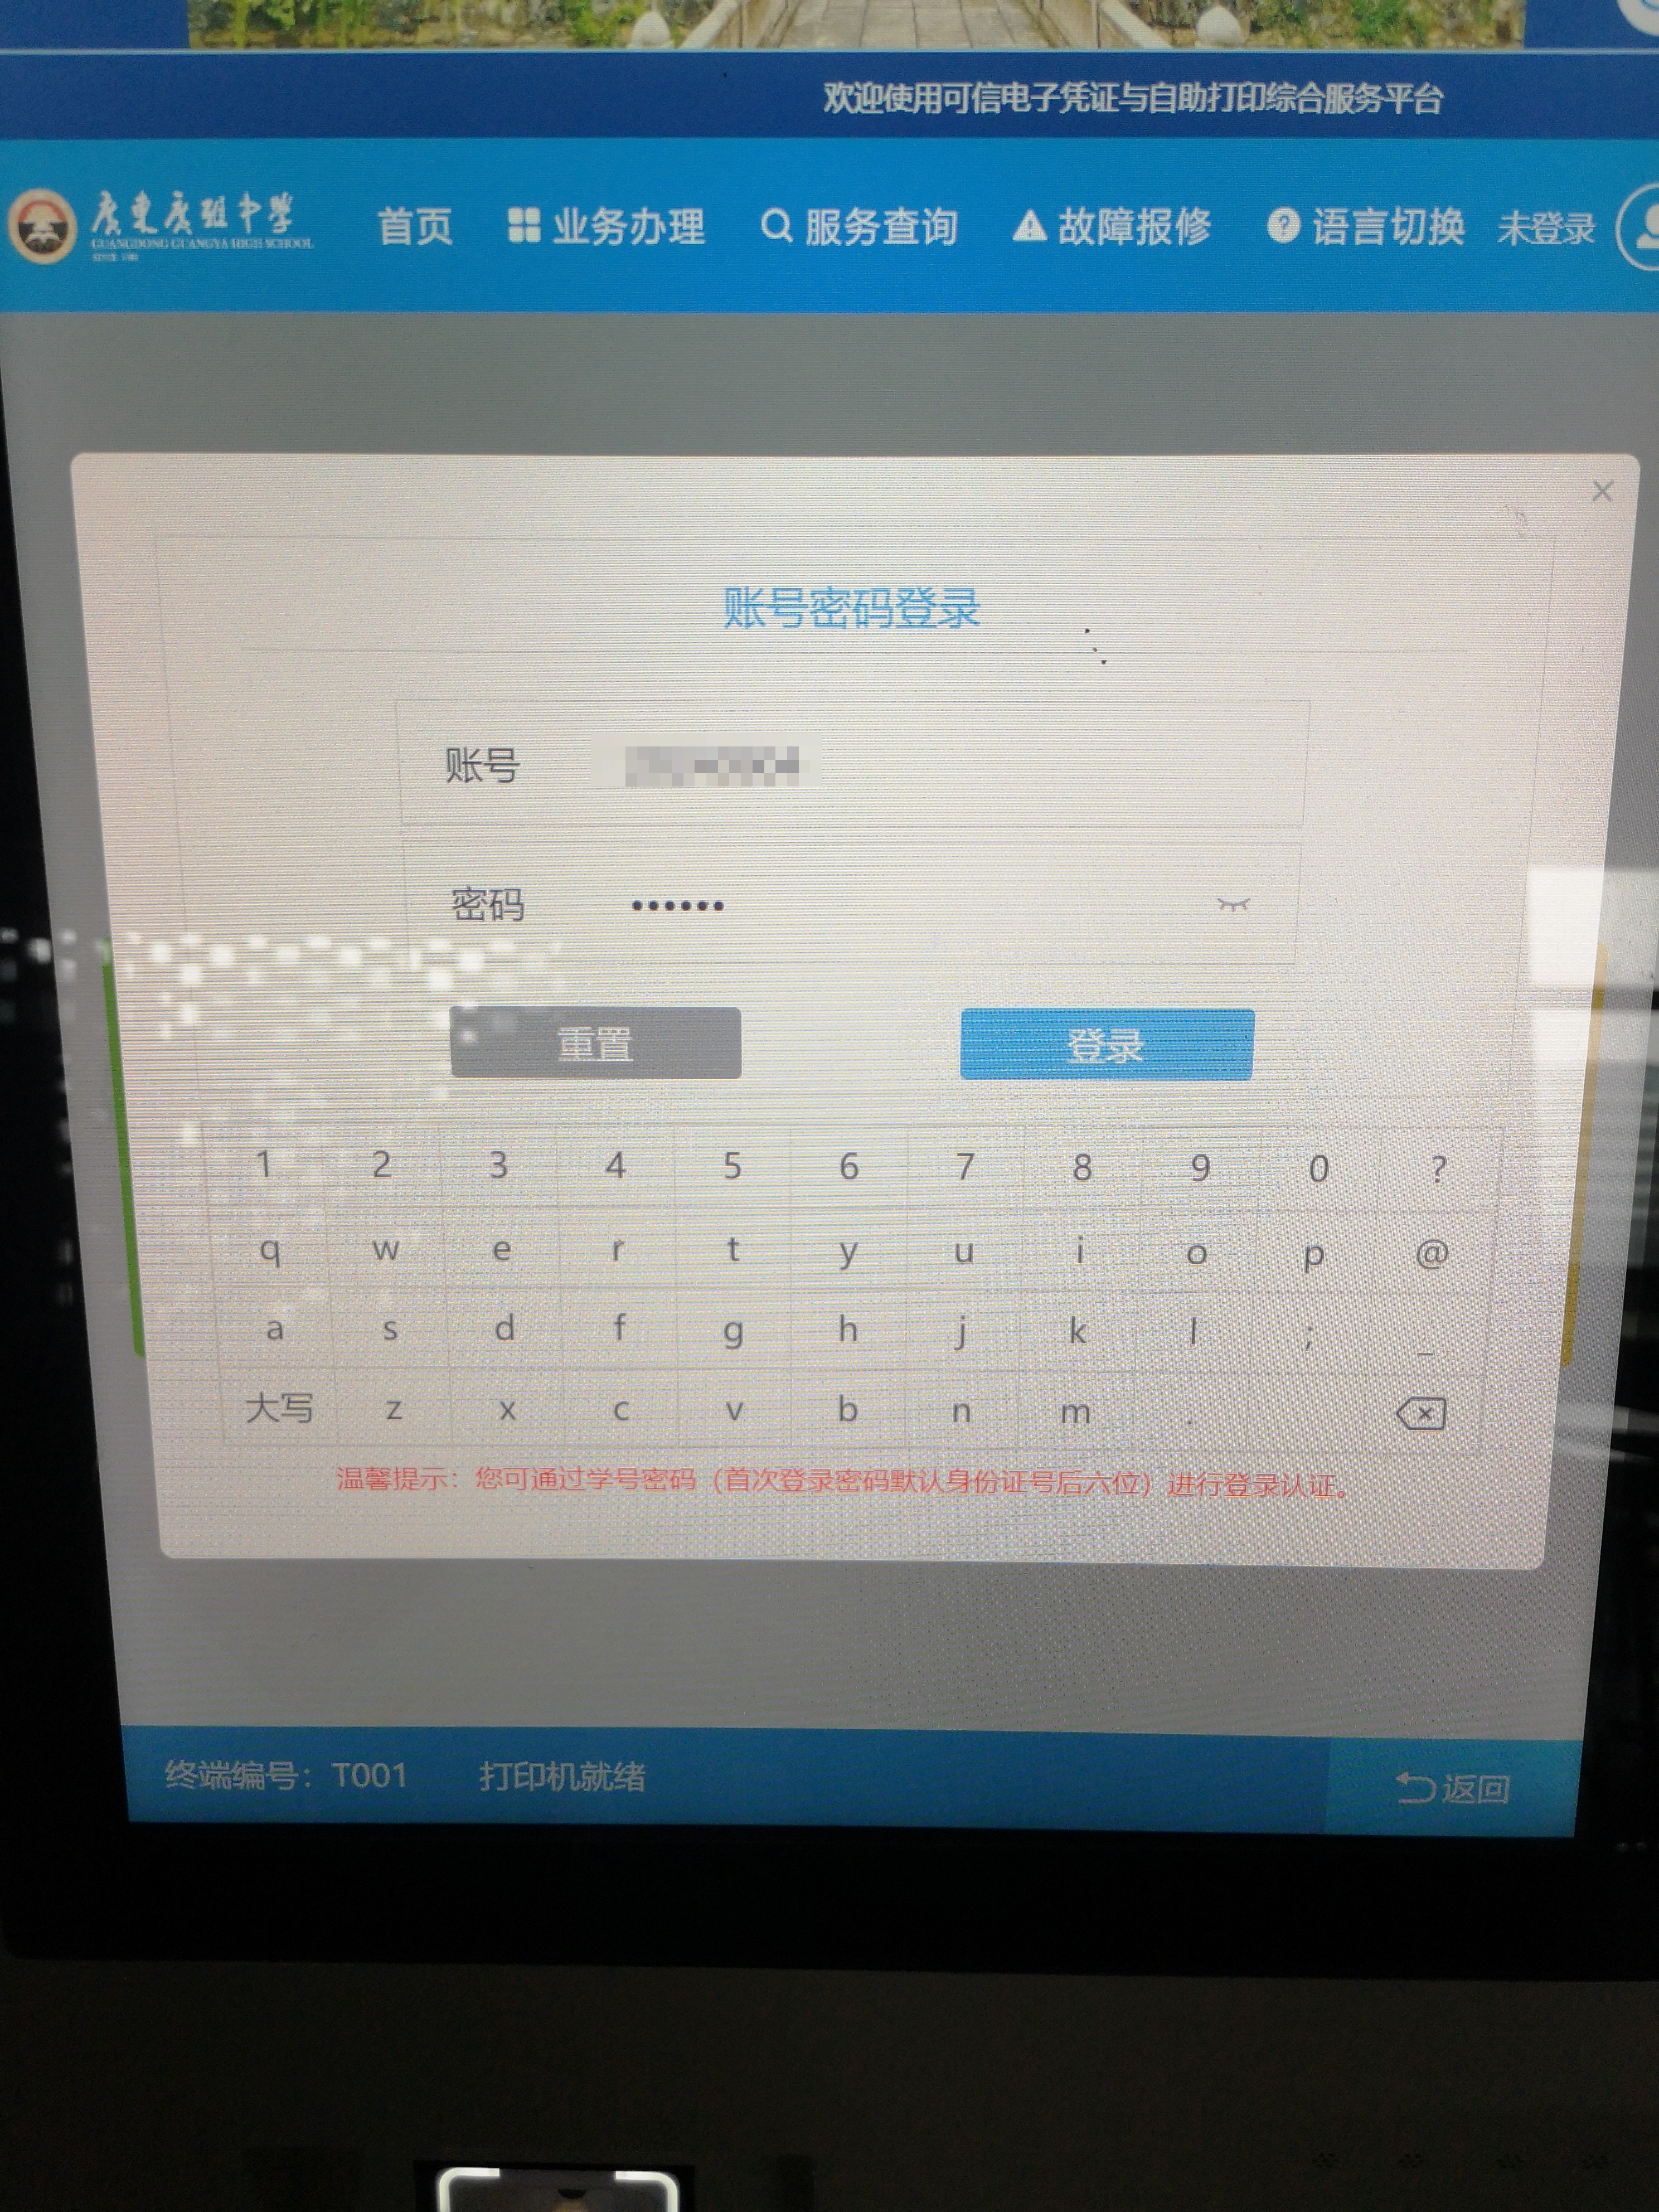
\includegraphics[width=\textwidth]{prove/prove4}
        \caption*{填写学号和身份证后6位}
        \label{fig:prove4}
      \end{minipage}
    \end{figure}
    然后，你就可以点击主页顶部菜单栏的“业务办理”，点击“中文成绩证明”，稍作等待，就能看到你的成绩证明了。
    \begin{figure}[ht]
      \centering
      \begin{minipage}{0.45\textwidth}
        \centering
        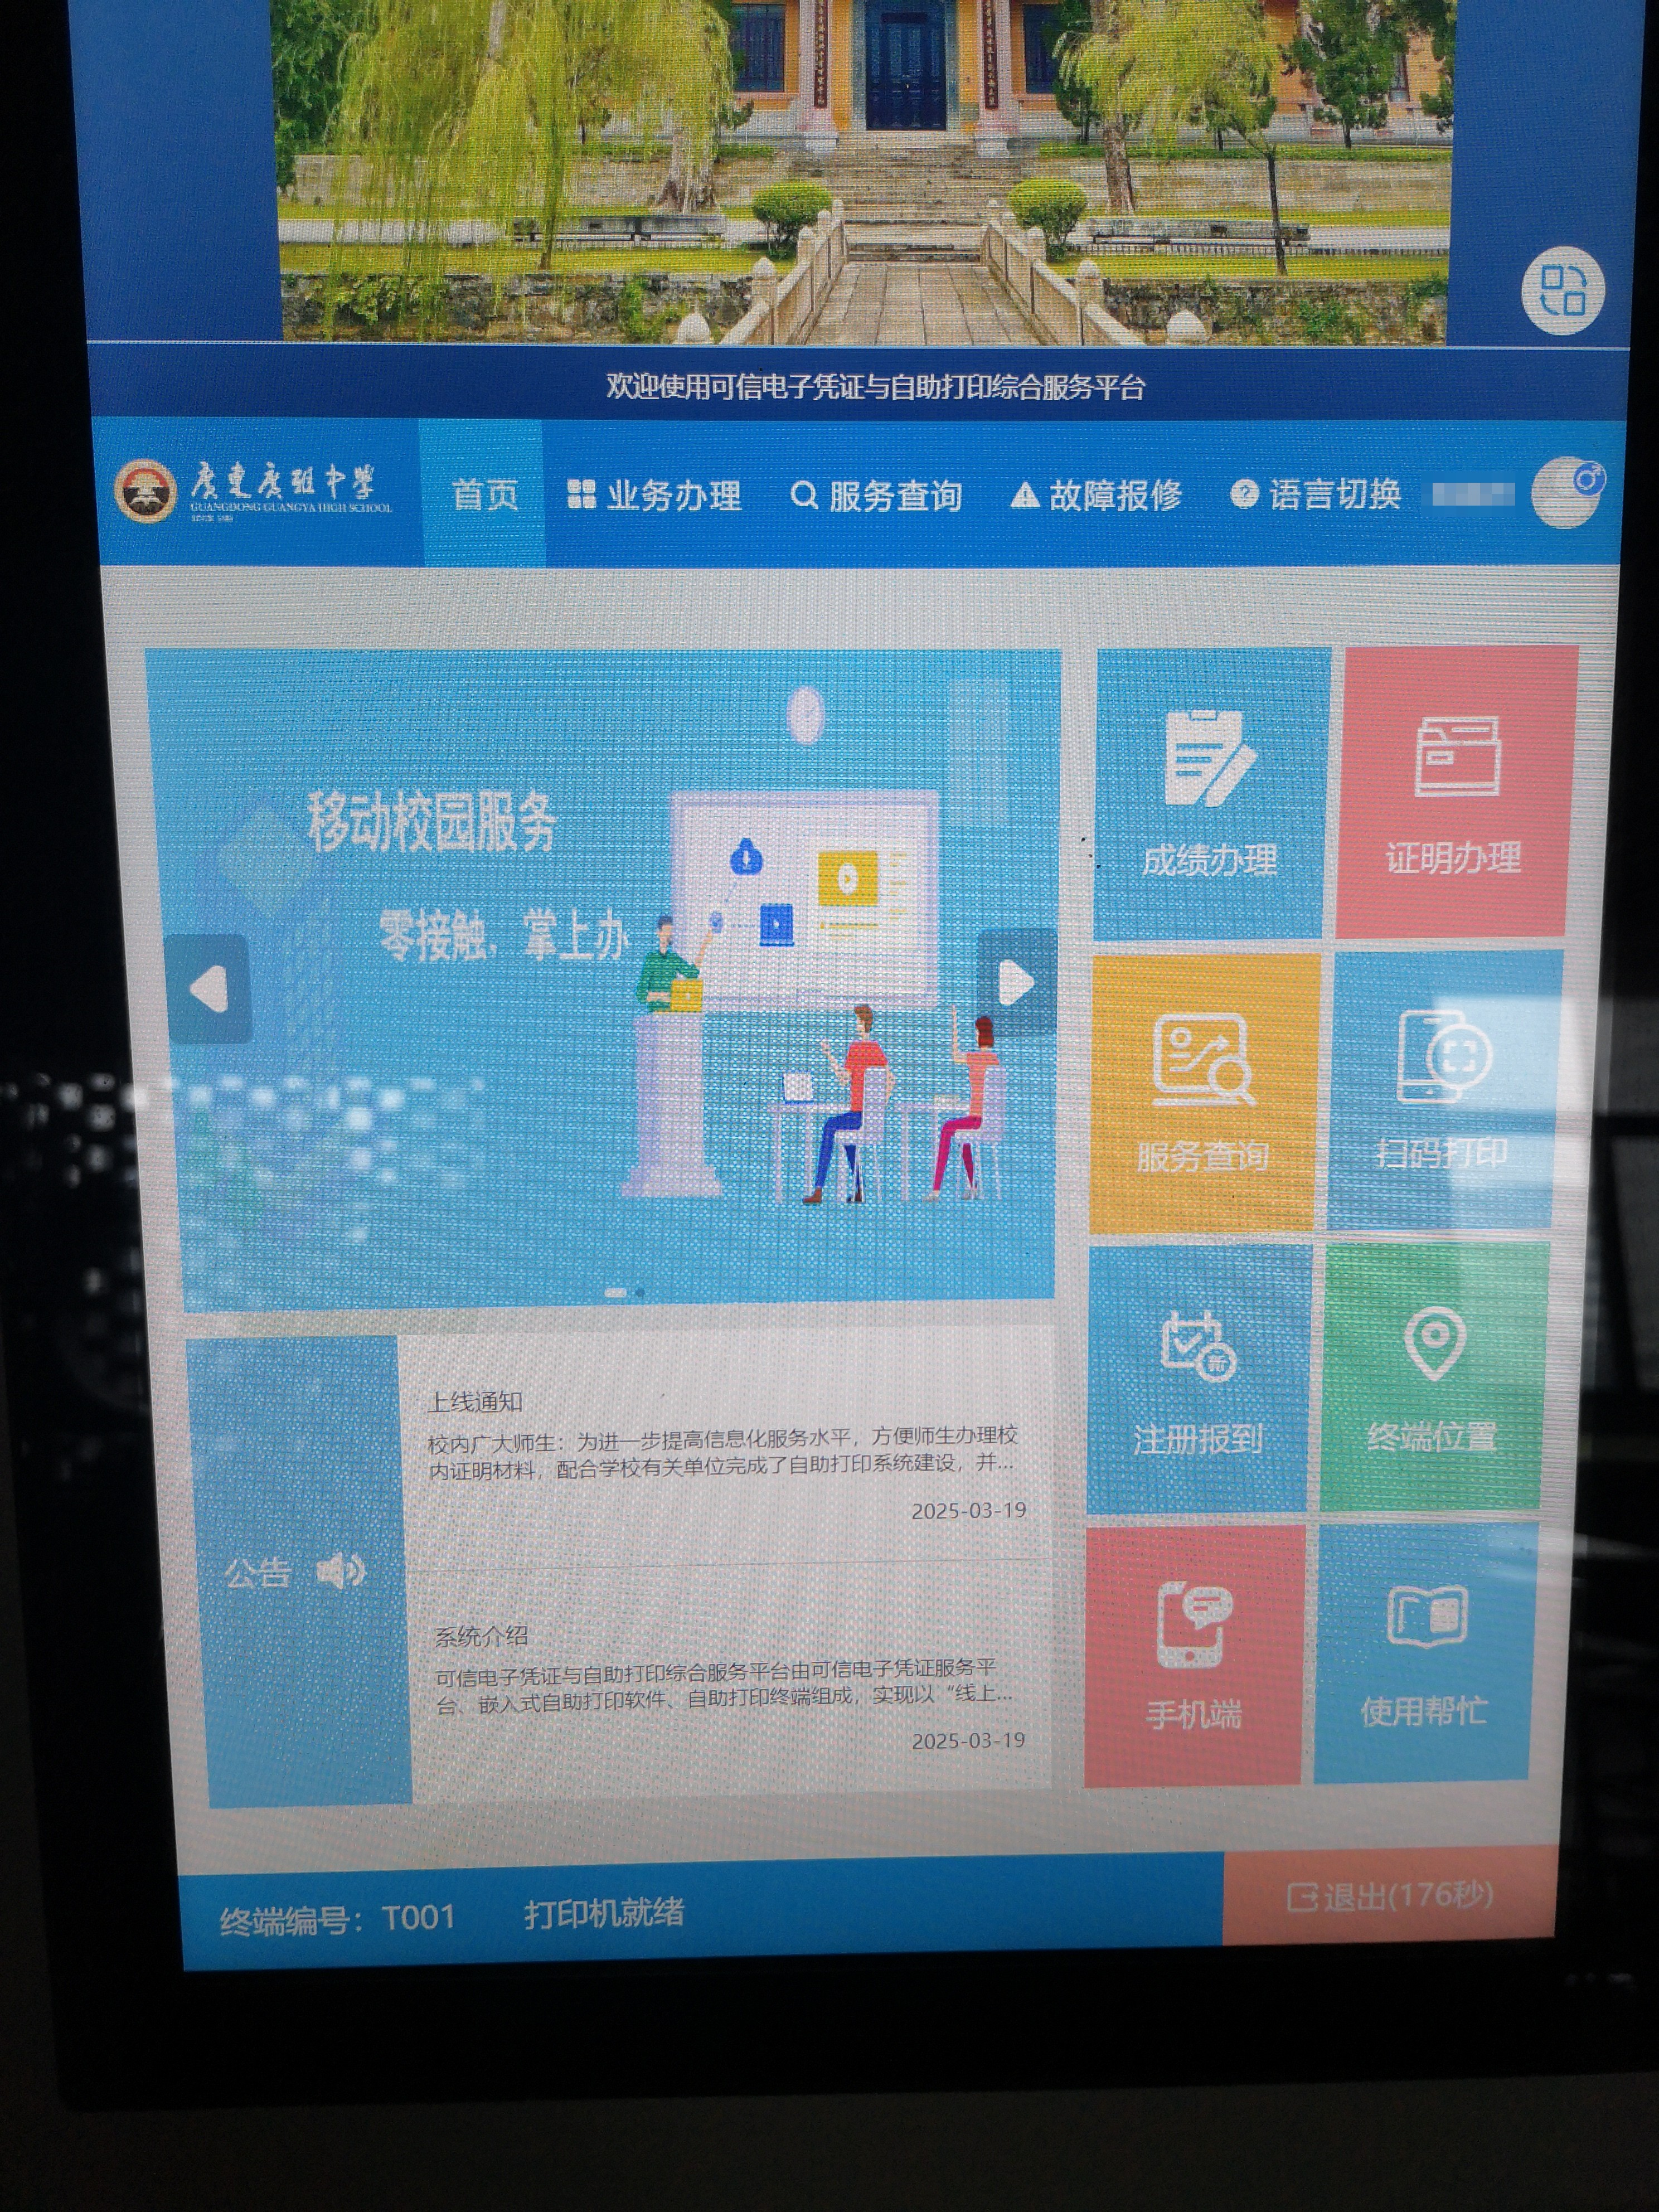
\includegraphics[width=\textwidth]{prove/prove5}
      \end{minipage}
      \hfill
      \begin{minipage}{0.45\textwidth}
        \centering
        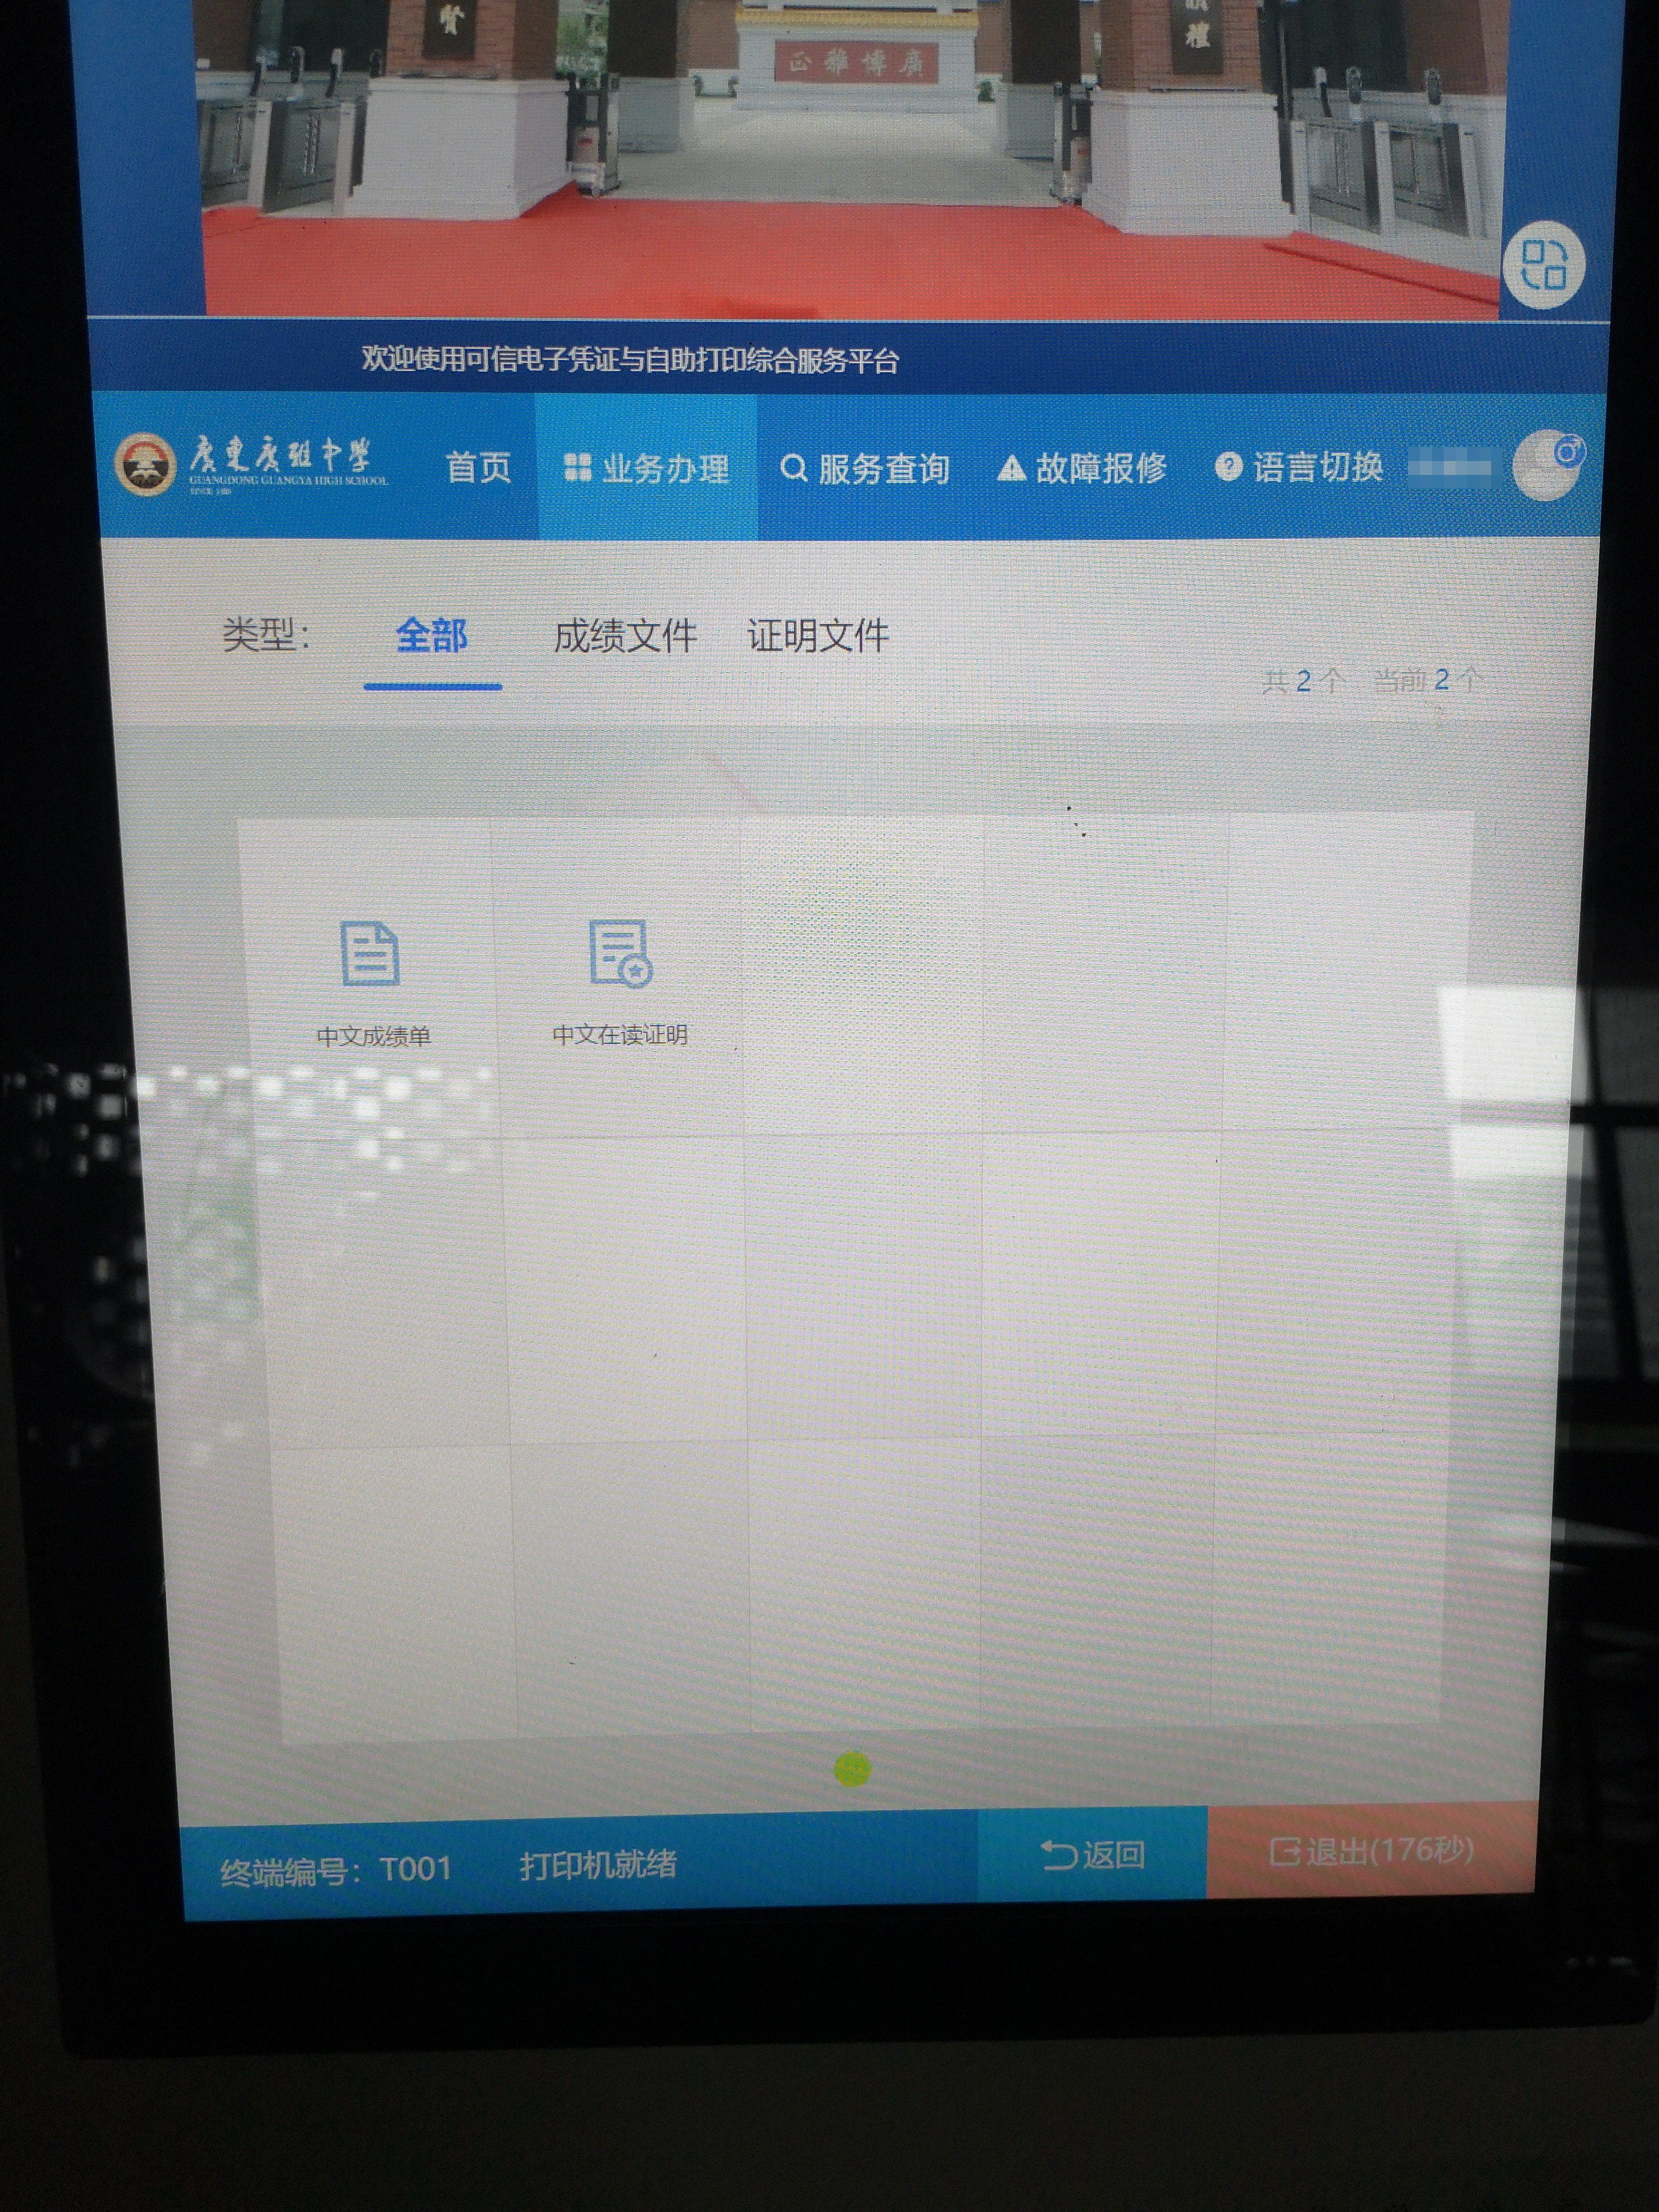
\includegraphics[width=\textwidth]{prove/prove6}
      \end{minipage}
      \caption{业务办理与中文成绩证明}
      \label{fig:prove56}
    \end{figure}
    然后，点击右边蓝色的打印机形状的按钮，就可以打印了，如\cref{fig:prove7}。每个学生可以免费打印10次。
    \begin{figure}[ht]
      \centering
      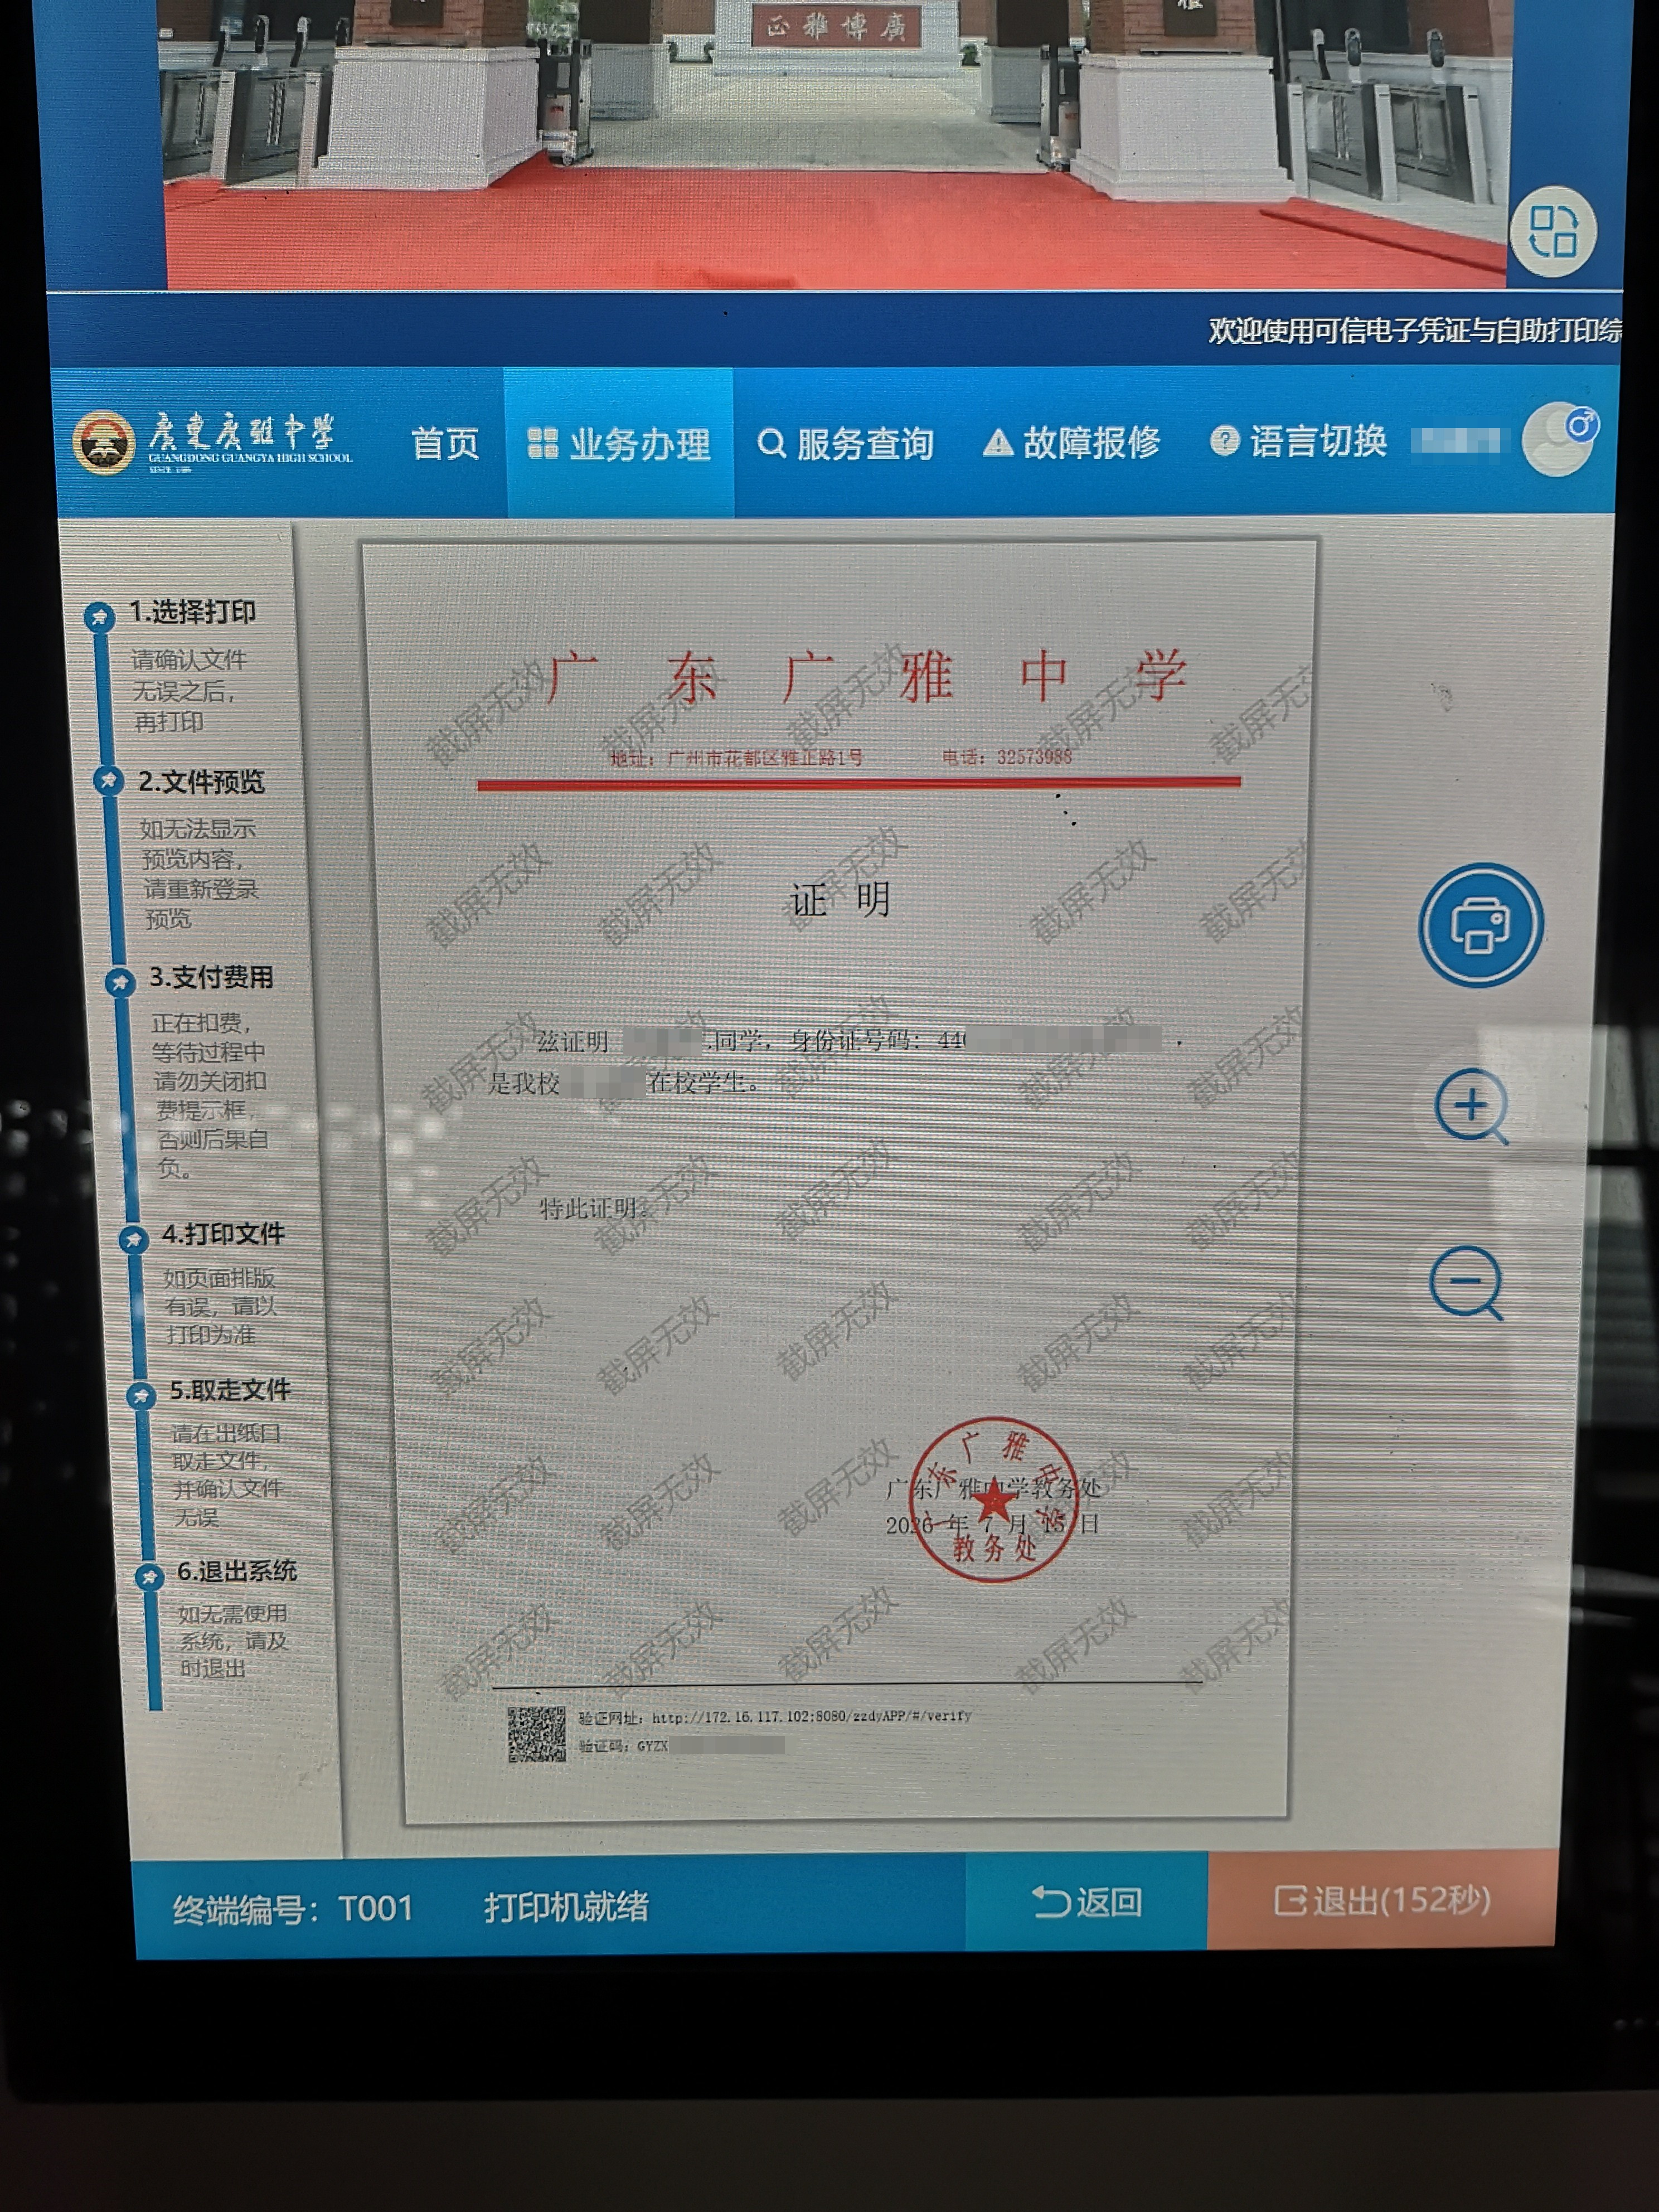
\includegraphics[width=0.45\textwidth]{prove/prove7}
      \caption{打印成绩证明}
      \label{fig:prove7}
    \end{figure}
    拿到打出来的纸质版成绩证明，就可以拿去尽情使用了。
